\documentclass[a4paper,11pt,english]{article} 

\usepackage[left=1in,right=1in,top=1in,bottom=1in]{geometry}
\usepackage[utf8]{inputenc} 
\usepackage[T1]{fontenc} 
\usepackage[english]{babel}
\usepackage{amsmath,amsthm,amsfonts,amssymb,amstext} 
\usepackage{textcomp}
\usepackage{upgreek} 
\usepackage[final]{graphicx}      
%\usepackage{epstopdf}
%\usepackage{float} 
%\usepackage[font=footnotesize,labelfont=bf,textfont=it]{caption} 
\usepackage[usenames,dvipsnames]{xcolor} 
%\usepackage{pdfpages} 
%\usepackage{siunitx}
%\captionsetup[figure]{name=Fig.} 
%\captionsetup[table]{name=Tab.} 
\usepackage[bookmarks=true,bookmarksnumbered=true]{hyperref}
%\usepackage[round]{natbib}
%\usepackage{smartdiagram}

\parindent 0cm 
\addtolength{\textheight}{0cm}
\addtolength{\voffset}{0cm} 
\setlength{\parskip}{0.6\baselineskip}

\begin{document}

\title{\textbf{The GALAH survey} \\ Update on spectroscpic analysis pipeline}
\author{WG4 - Sven Buder, contributions by Anish Amarsi, Jane Lin, Karin Lind, Thomas Nordlander}

\maketitle

\section{Important changes after GALAH DR2}

\subsection{Spectroscopic synthesis pipeline available for members}

The pectroscopic synthesis pipeline is now open for all GALAH members to use via

\url{https://galah-survey.org/wiki/galah-spectrum-synthesis-pipeline}

\subsection{Documents in preparation of GALAH DR3 available on github}

Initial documents for the preparation of GALAH DR3 have been uploaded on a private (hidden) repository on

\url{https://github.com/svenbuder/GALAH_DR3}

If you want to access to these documents, please email Sven to be added as a collaborator (you need a github account for this).

\subsection{Updates regarding SME}

\begin{itemize}
\item Pipeline finally and successfully converted to the recent SME version 536 (if interested, ask WG4 regarding the major changes). Thanks to Thomas Nordlander!
\item Improved continuum selection and normalisation with SME. Thanks to Karin Lind!
\item Non-LTE now also for H (in addition to Li, O, Na, Mg, Al, Si, and Fe). Thanks to Anish Amarsi!
\end{itemize}

\subsection{Updates regarding use of \textit{Gaia} DR2 and asterseismic data}

\begin{figure}[!ht]
\centering
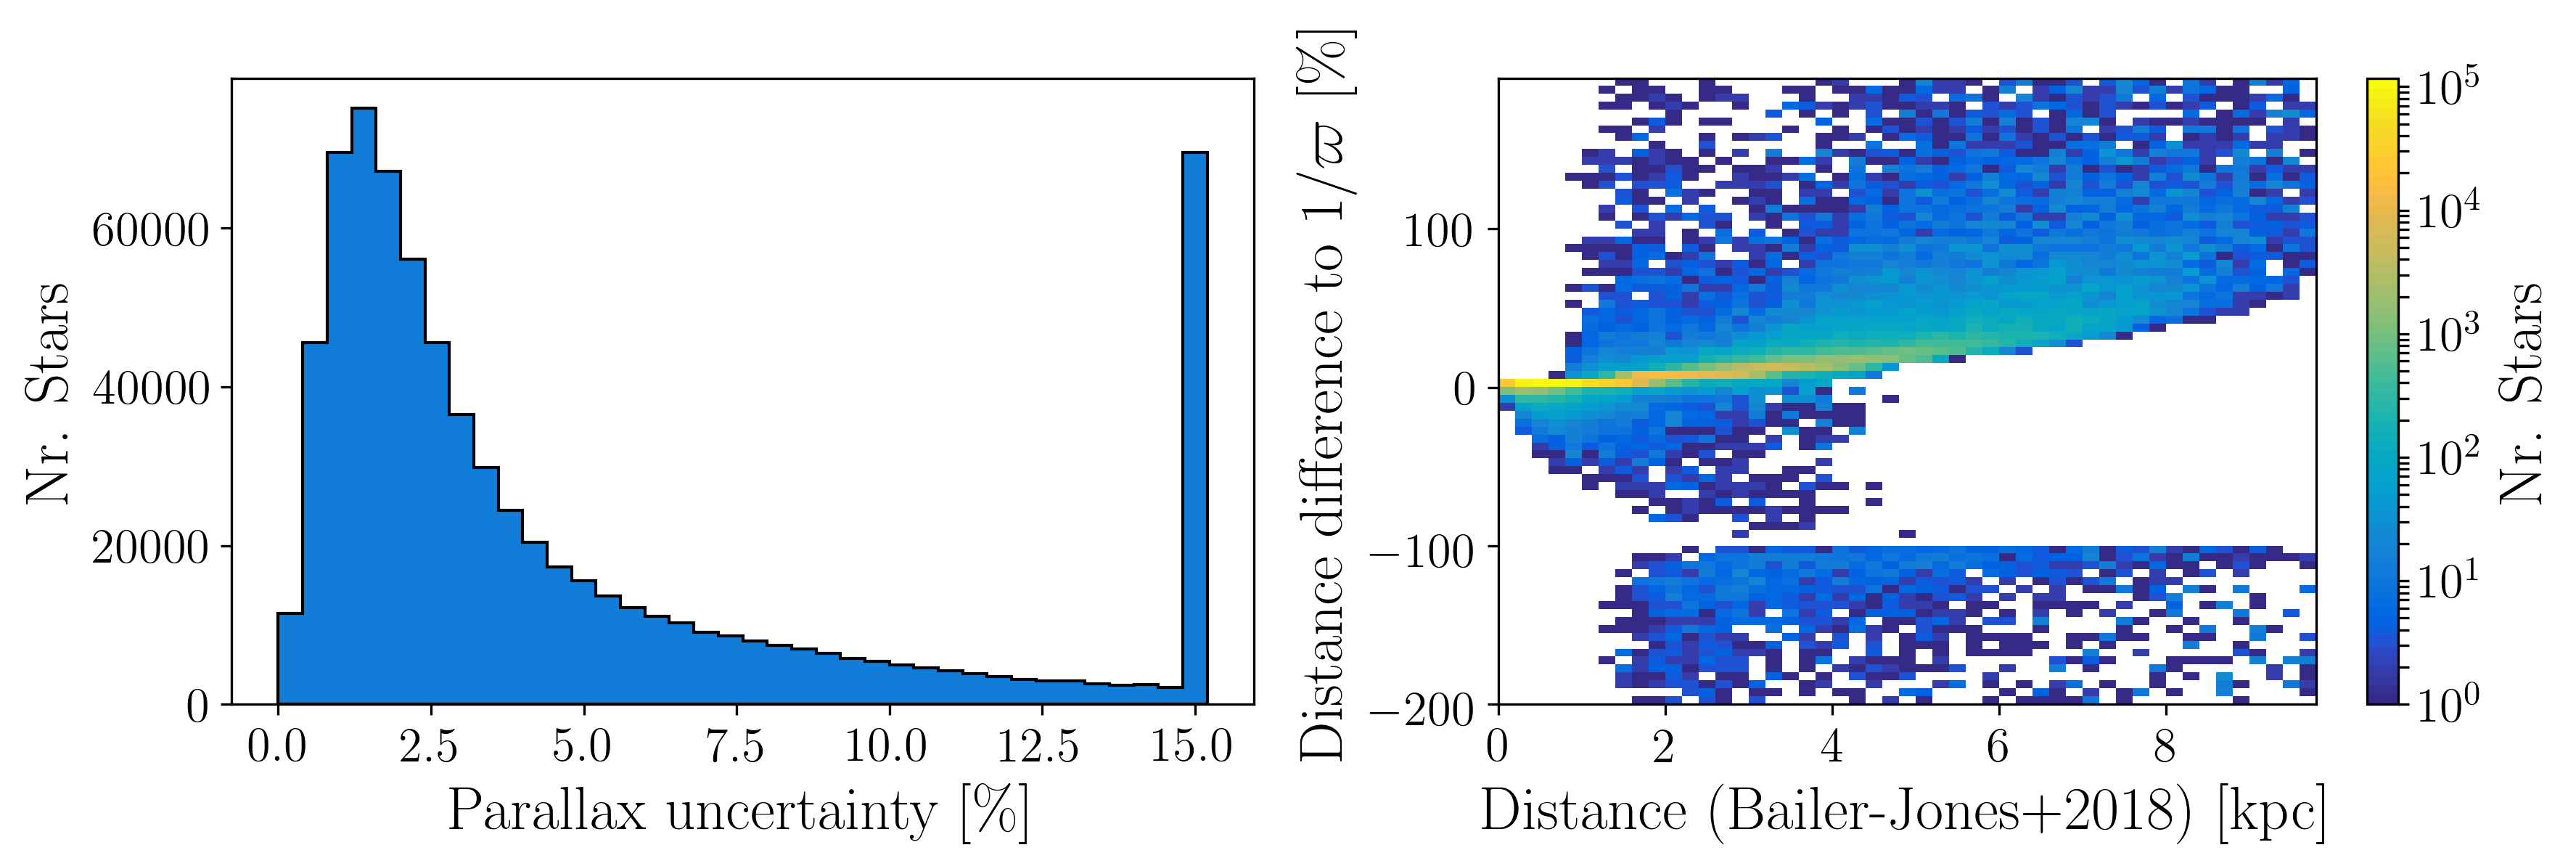
\includegraphics[width=\textwidth]{../../input/figures/parallax_uncertainties.png}
\caption{Overview of parallaxes/distances of the stars observed by GALAH.}
\label{fig:parallax_overview}
\end{figure}

\begin{itemize}
\item Parallaxes now available for almost all stars observed by GALAH and a vast majority of them are very good, see \autoref{fig:parallax_overview}
\item The asteroseismic information provided by Sanjib Sharma and others have been used to run a pipeline version which constrains $\log g$ as a function of $T_\text{eff}$ and $\nu_\text{max}$, which consists of up to 3175 stars (including bad S/N, bad $\nu_text{max}$ values, and bad reductions).
\item For the interim mass and age estimation, we have switched to the use of Parsec isochrones, which include core helium burning stars (in contrary to Dartmouth isochrones) and alpha-enhancement (in contrary to MIST). Thanks to Jane Lin!
\end{itemize}

\section{Performances}

\subsection{\textit{Gaia} FGK benchmark stars}

We do not see any significant biases for Teff and logg, but had to correct and [Fe/H] bias of -0.1 (underestimated [Fe/H]), see \autoref{fig:gbs_performance}. Underestimated temperatures for the hottest stars are still likely, but more testing is needed as the continuum normalisation has been improved and hydrogen has been implemented in non-LTE now.

\begin{figure}[!ht]
\centering
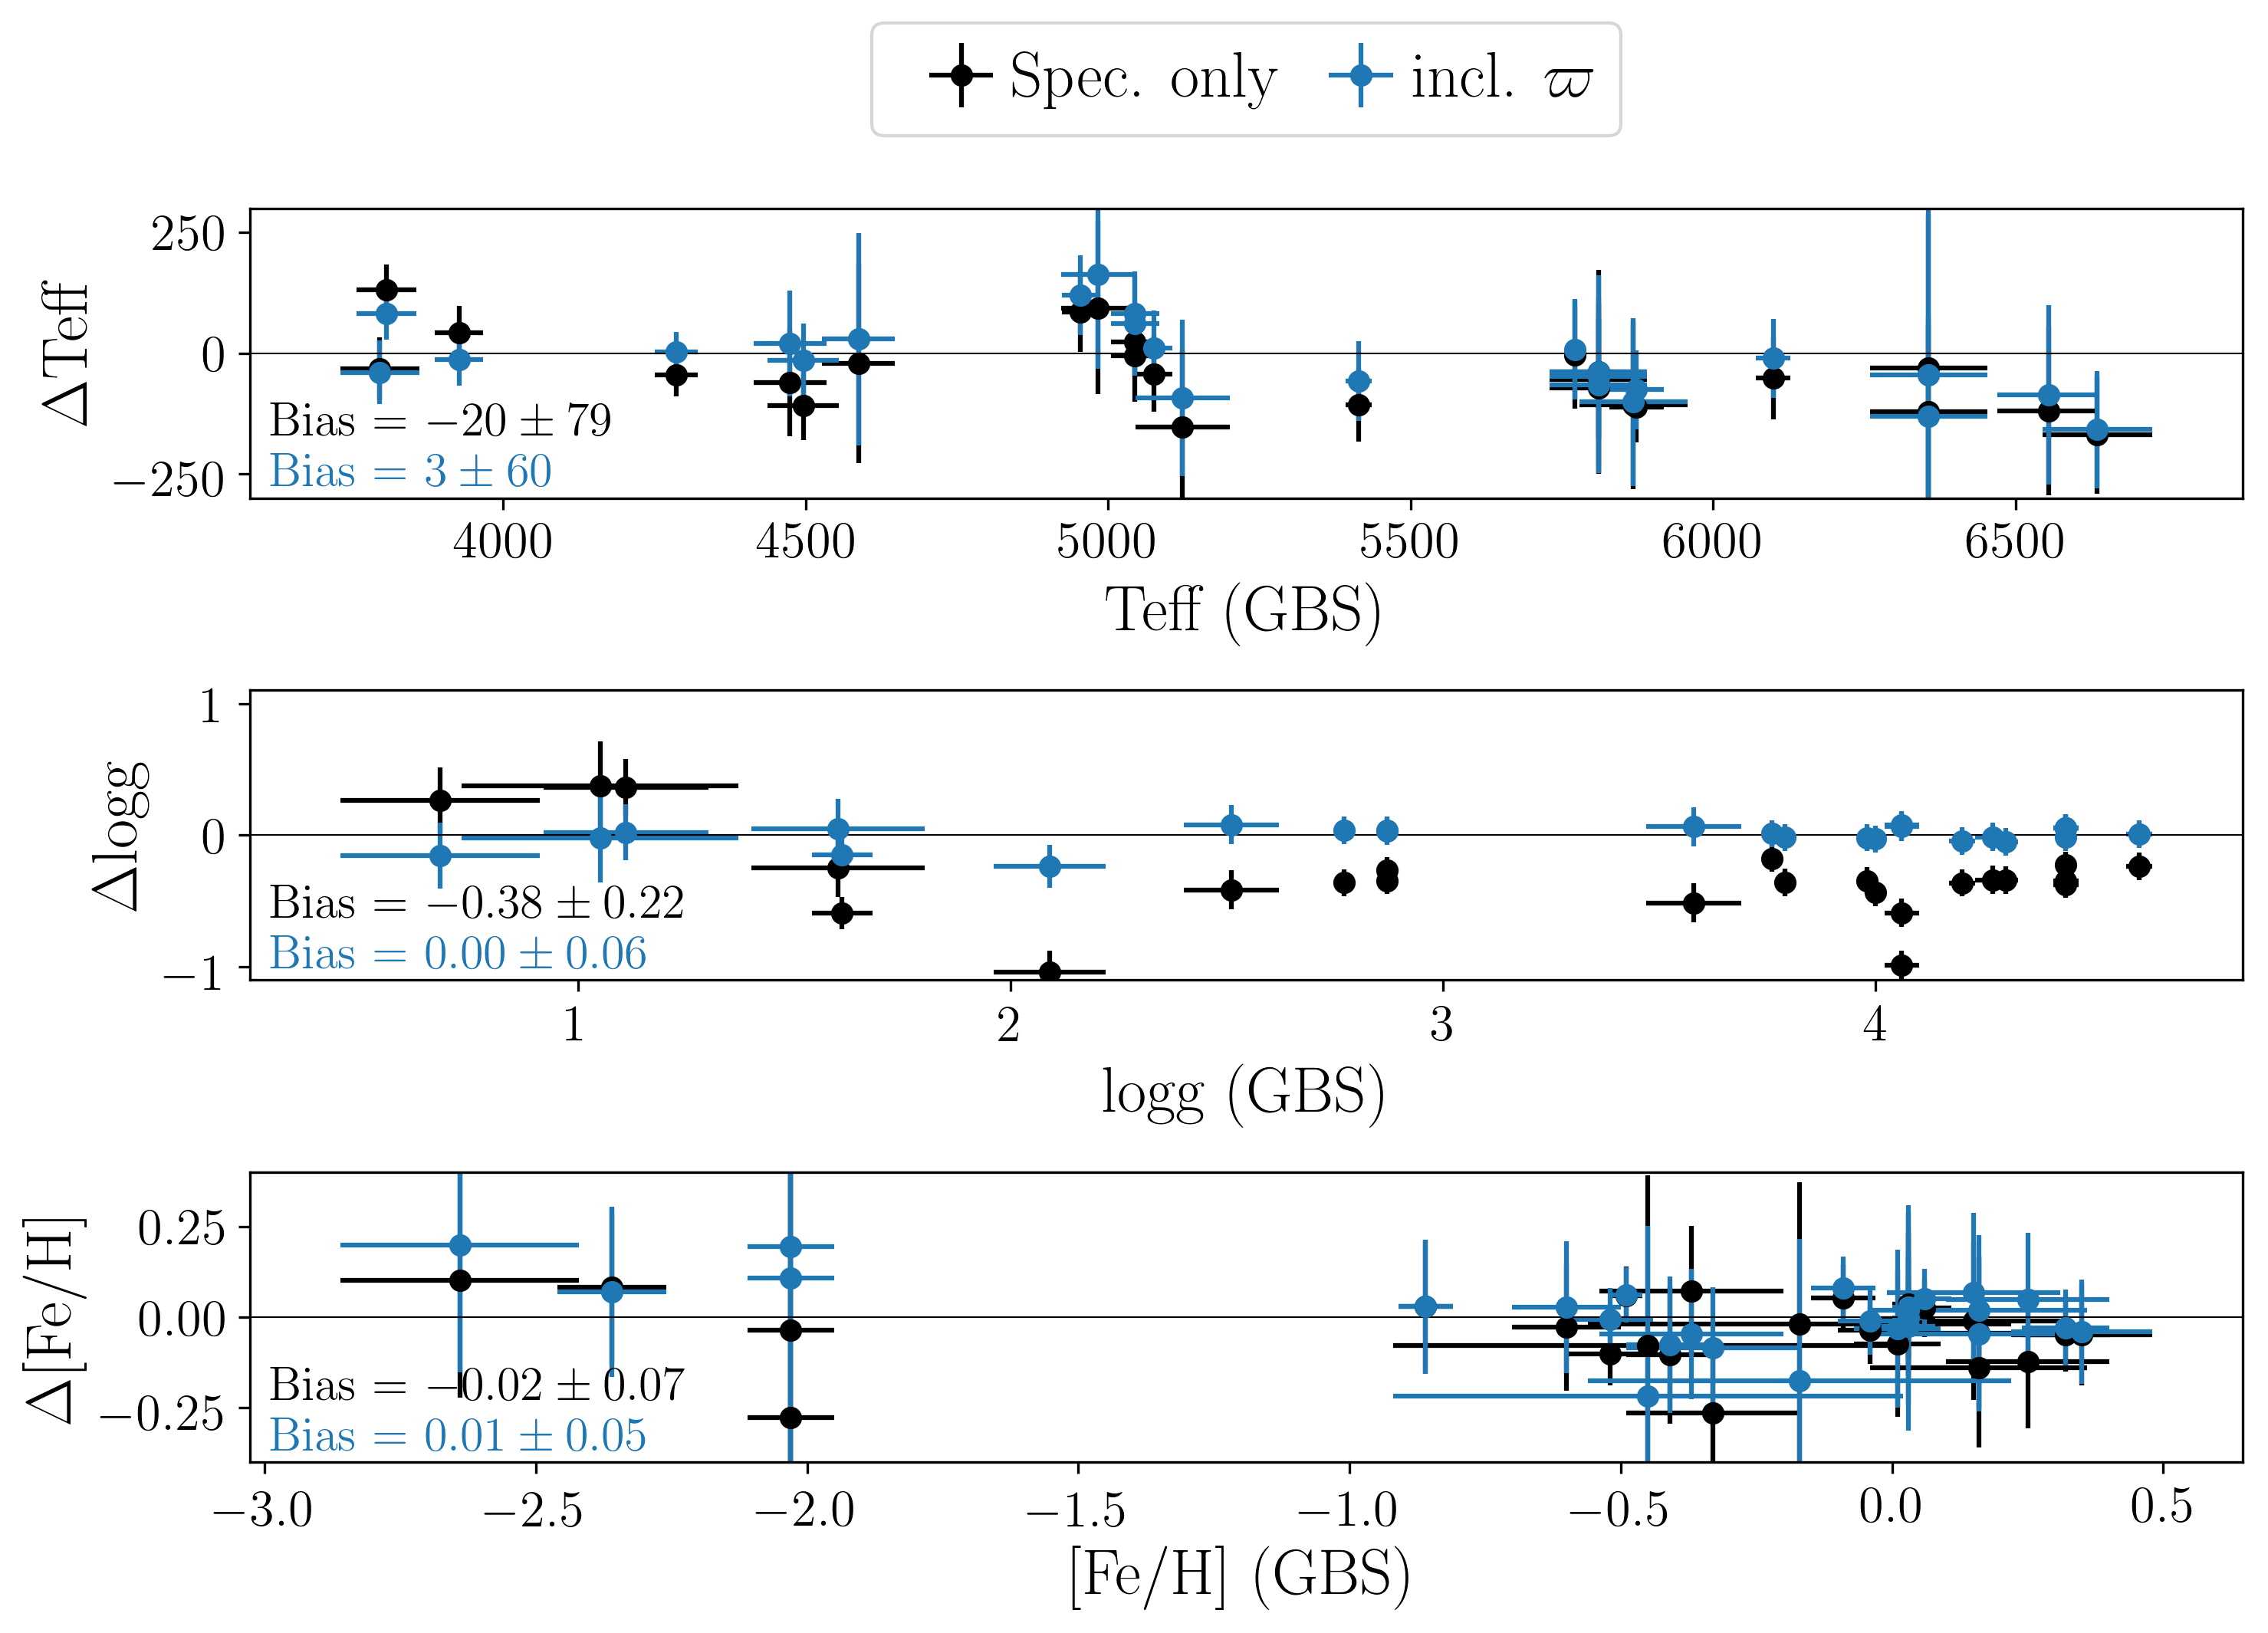
\includegraphics[width=\textwidth]{../../gbs/figures/gbs_performance_free_lbol.png}
\caption{Performance of GALAH synthesis pipeline without (black) and with (blue) bolometric information.}
\label{fig:gbs_performance}
\end{figure}

\subsection{Stars with asteroseismic information}

The overlap of the stars with asteroseismic parameters and parallaxes show that the bolometric pipeline (middle panels) performs significantly better than the pipeline without additional non-spectroscopic information (left panels). Especially the Red Clump stars show an outstanding agreement with the pipeline results which also used $\nu_\text{max}$ values, see \autoref{fig:seis_comparison1}.

\begin{figure}[!ht]
\centering
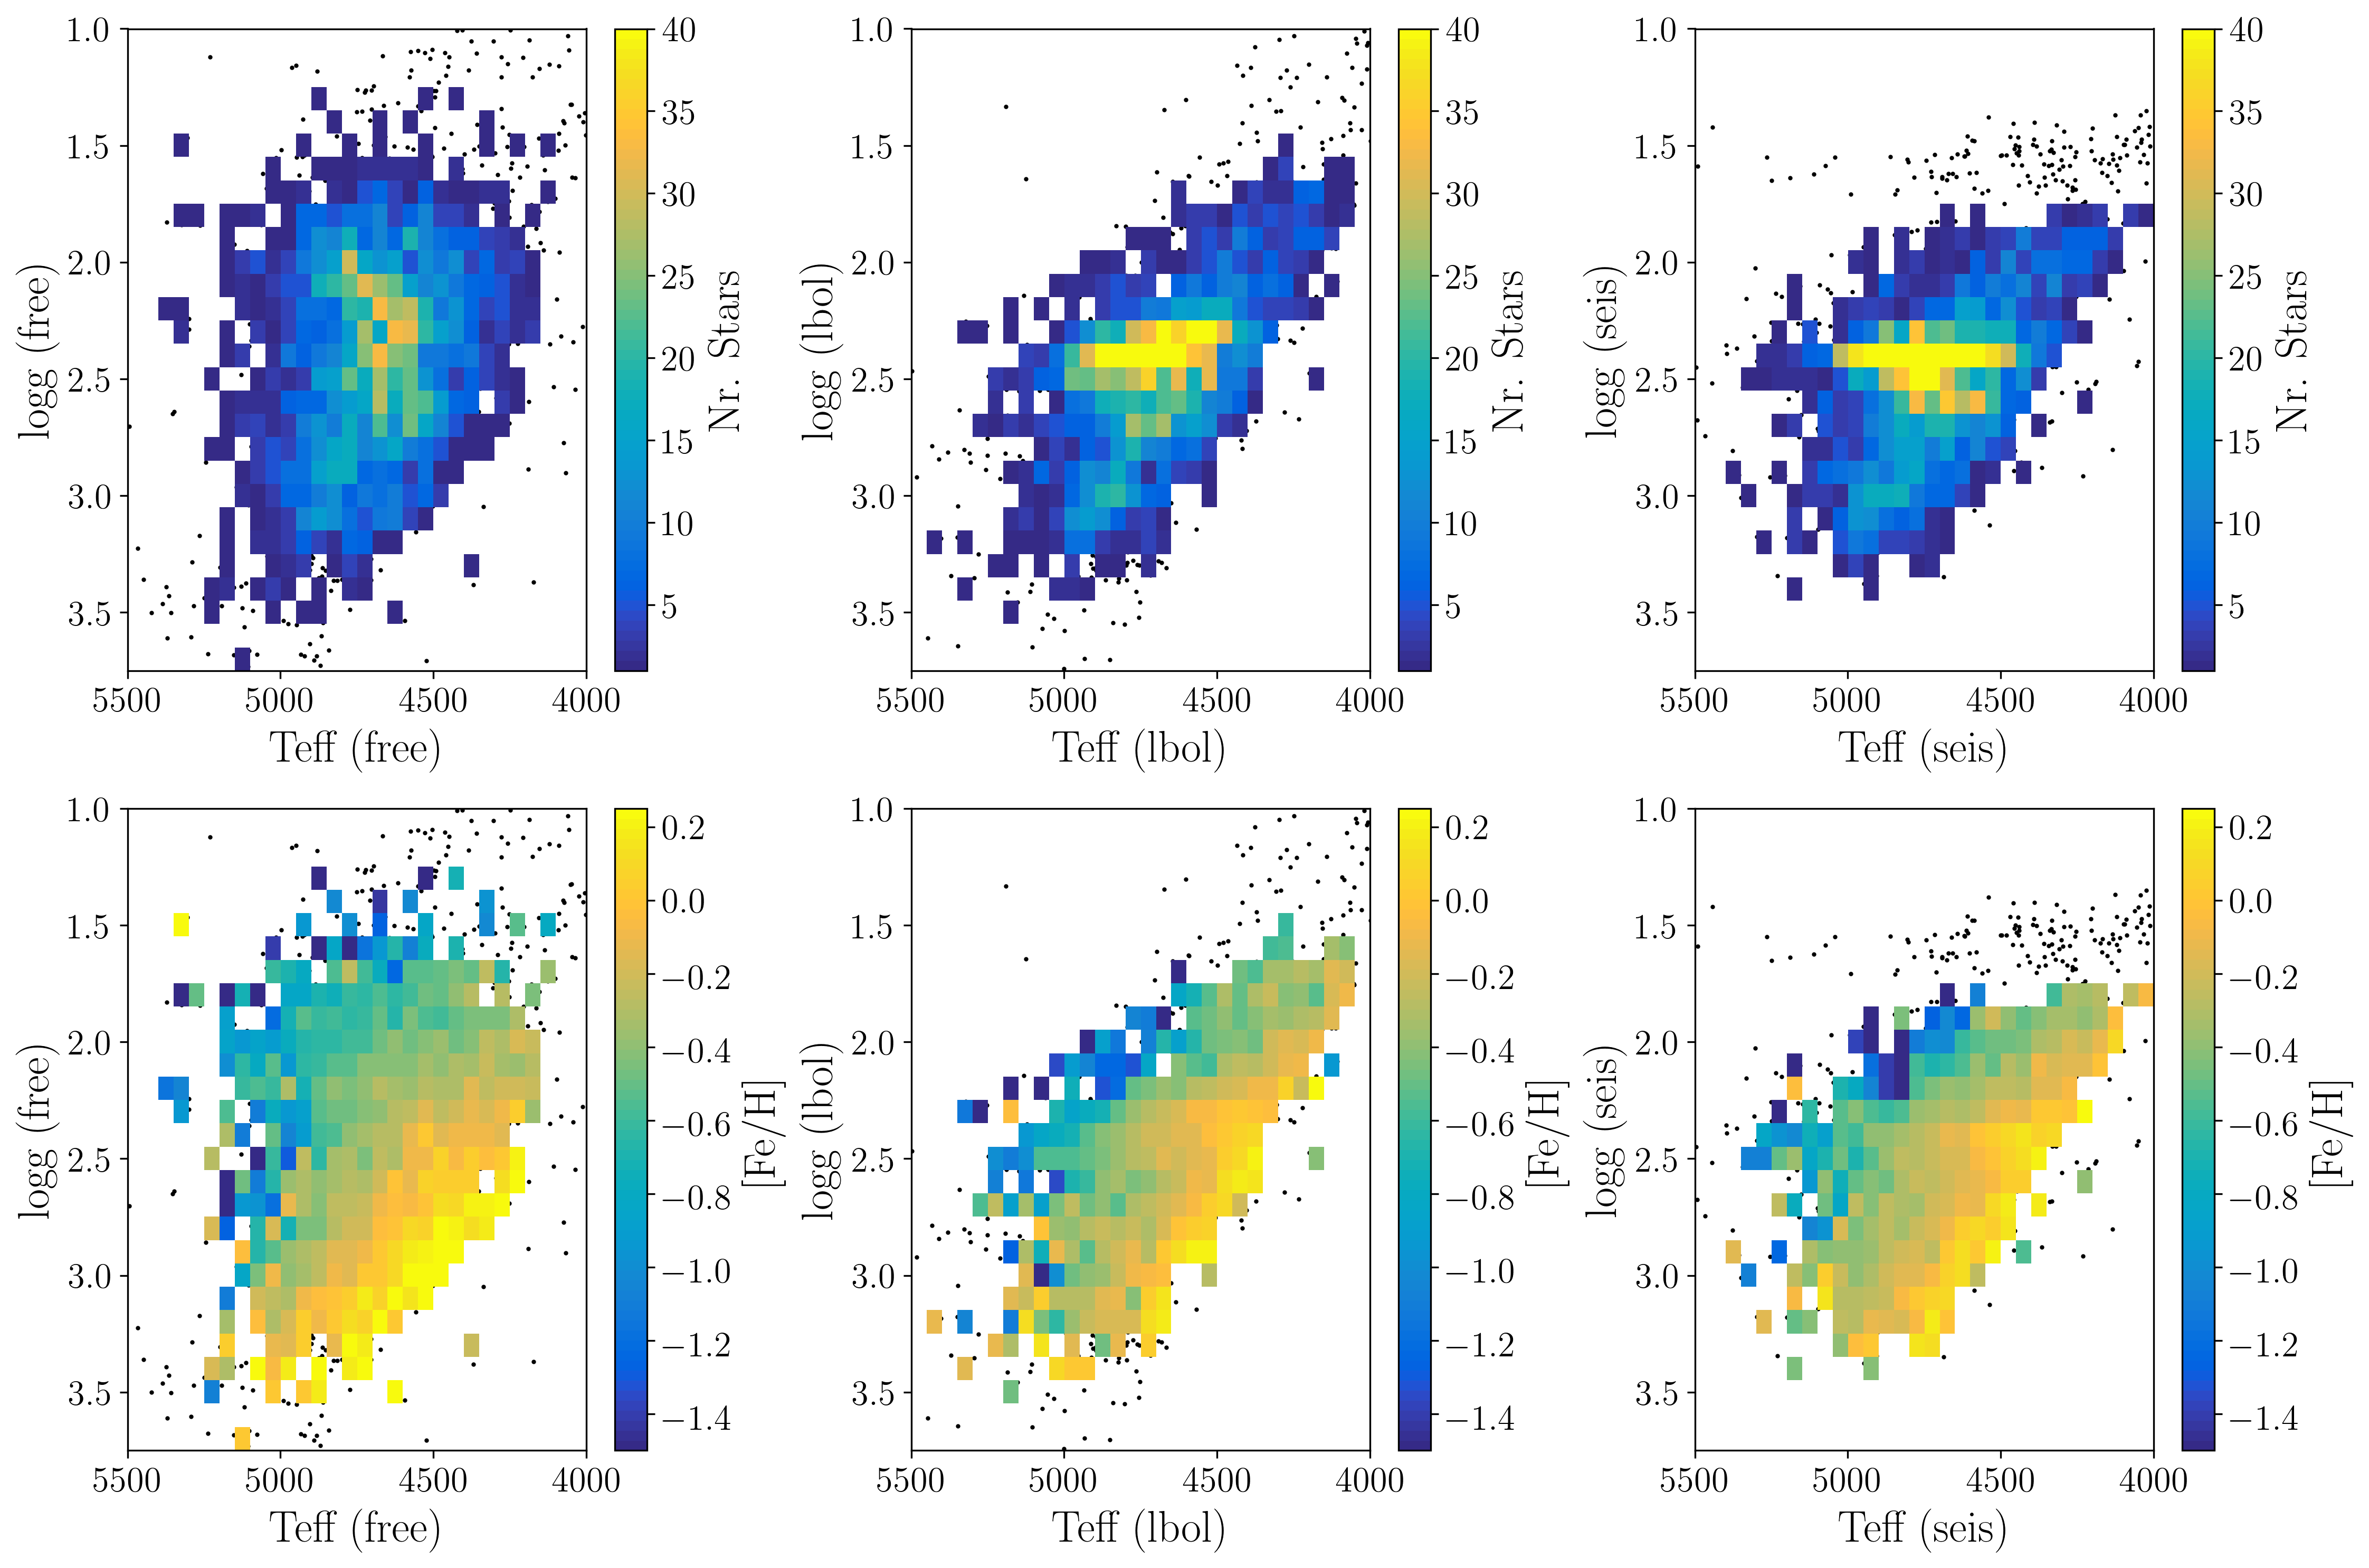
\includegraphics[width=\textwidth]{../../seis/figures/seis_comparison_3setups.png}
\caption{Kiel diagrams showing the performances of the three GALAH synthesis pipelines for the stars with asteroseismic information ($\log g = f(T_\text{eff}, \nu_\text{max})$) and bolometric information ($\log g = f(M, T_\text{eff}, \varpi, BC, K_S, A_{K_S})$), with top plots for density and bottom plots colored by mean [Fe/H]. Left panels show the results without additional non-spectroscopic information, middle panels when using bolometric information and right panels when using asteroseismic information.}
\label{fig:seis_comparison1}
\end{figure}

The scatter in the differences between asteroseismic and bolometric pipeline for logg is mainly driven by the red clump stars, which have to be further investigated, but are significantly better than for GALAH DR2, see the right hand plot in \autoref{fig:seis_comparison2}.

\begin{figure}[!ht]
\centering
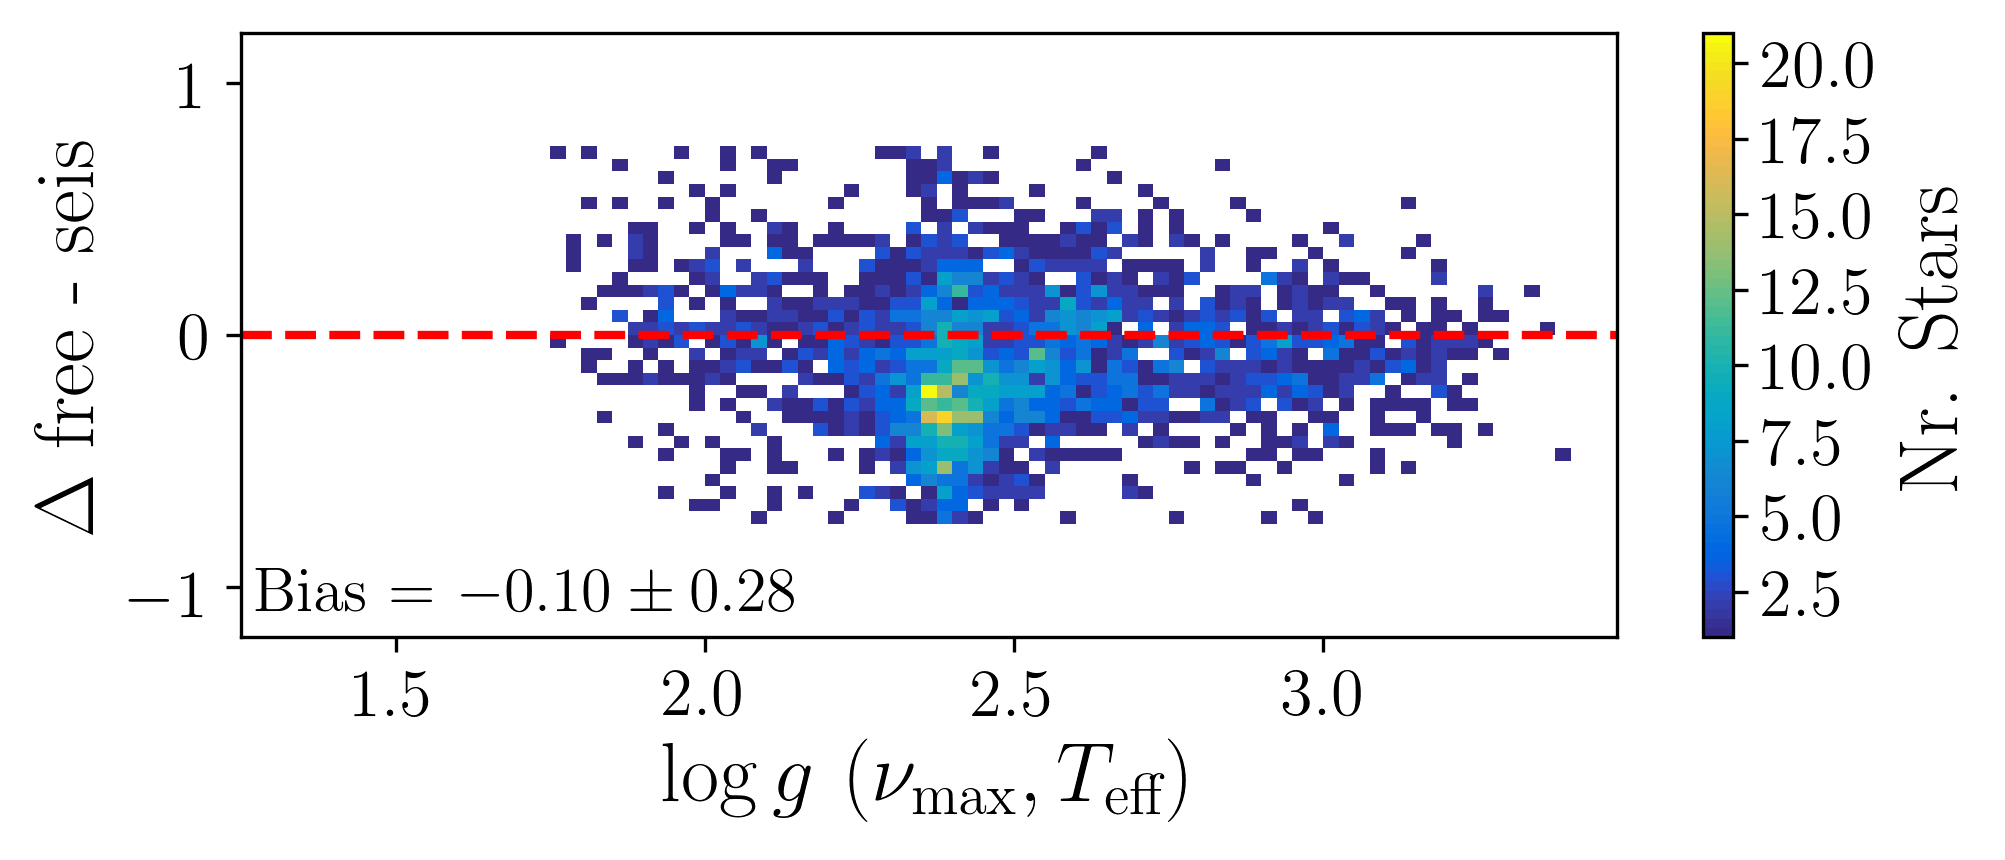
\includegraphics[width=0.49\textwidth]{../../seis/figures/seismic_sample_delta_free.png}
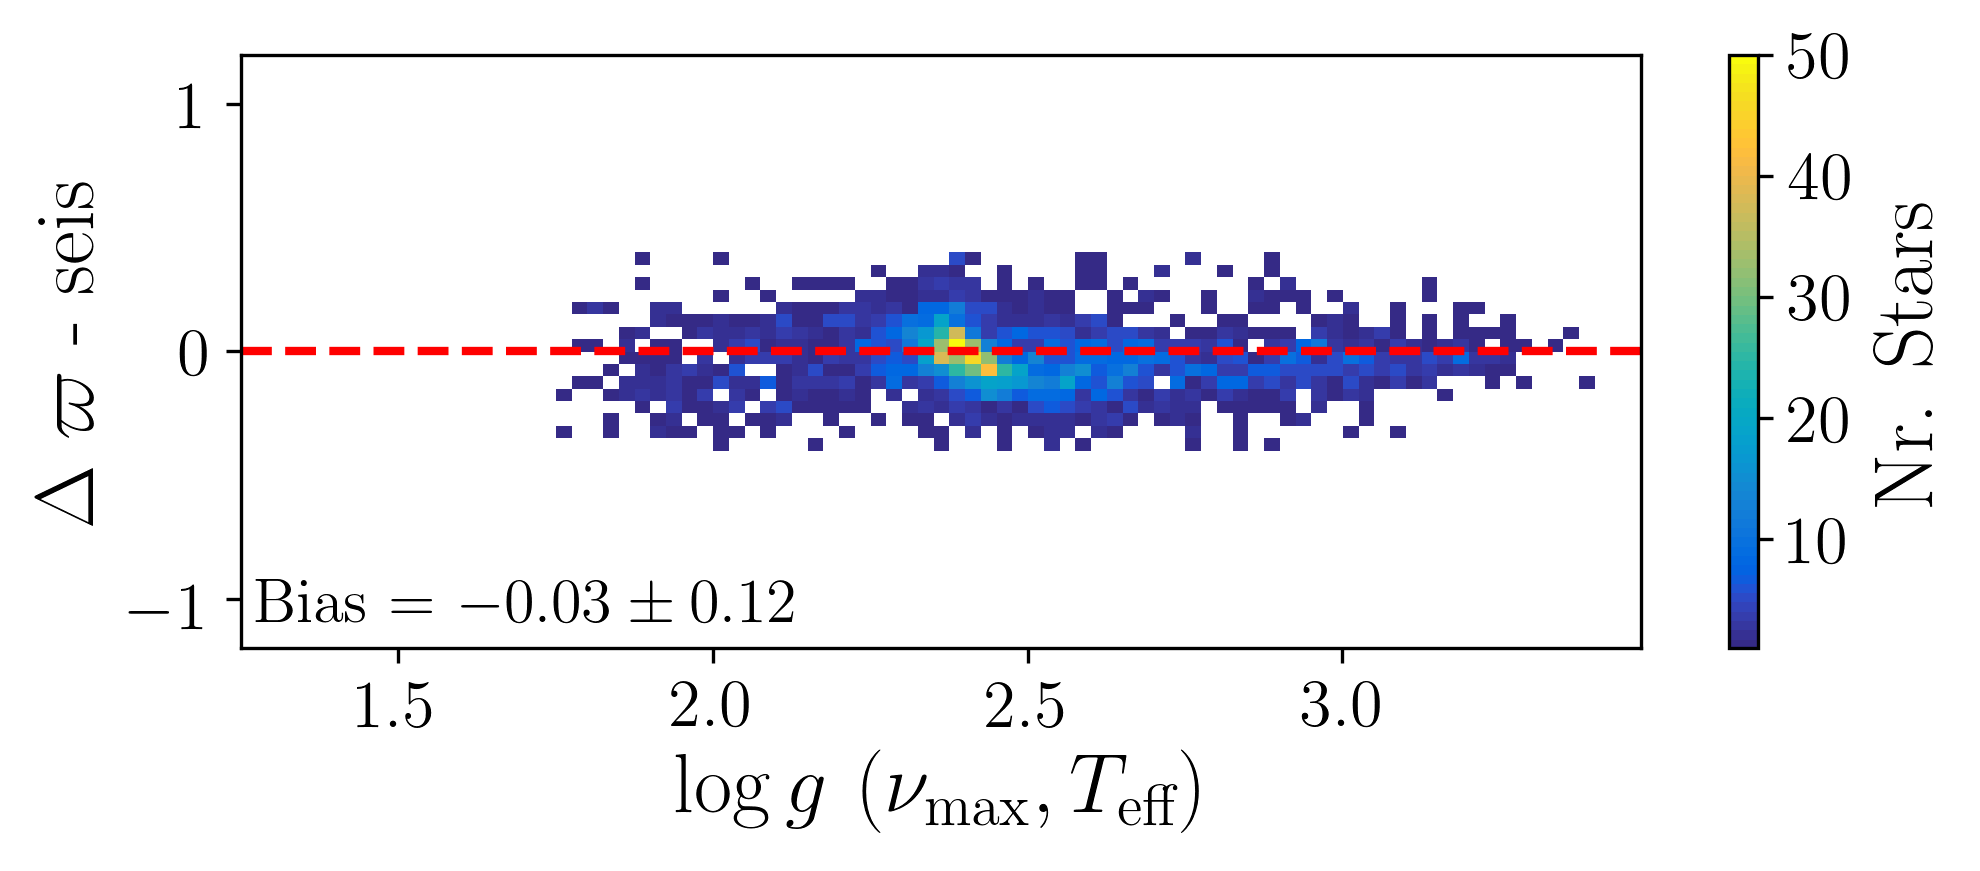
\includegraphics[width=0.49\textwidth]{../../seis/figures/seismic_sample_delta_lbol.png}
\caption{Difference of $\log g$ for stars with asteroseismic sample. Left: $\log g$ (free - seis). Right: $\log g$ (lbol - seis)}
\label{fig:seis_comparison2}
\end{figure}

The biases between asteroseismic and bolometric pipelines for the stellar parameters are not significant but show a trend of lower Teff (-21K), lower logg (-0.03dex), and lower [Fe/H] (-0.03dex) than the values from the pipeline using asteroseismic values/relations for logg.

\begin{figure}[!ht]
\centering
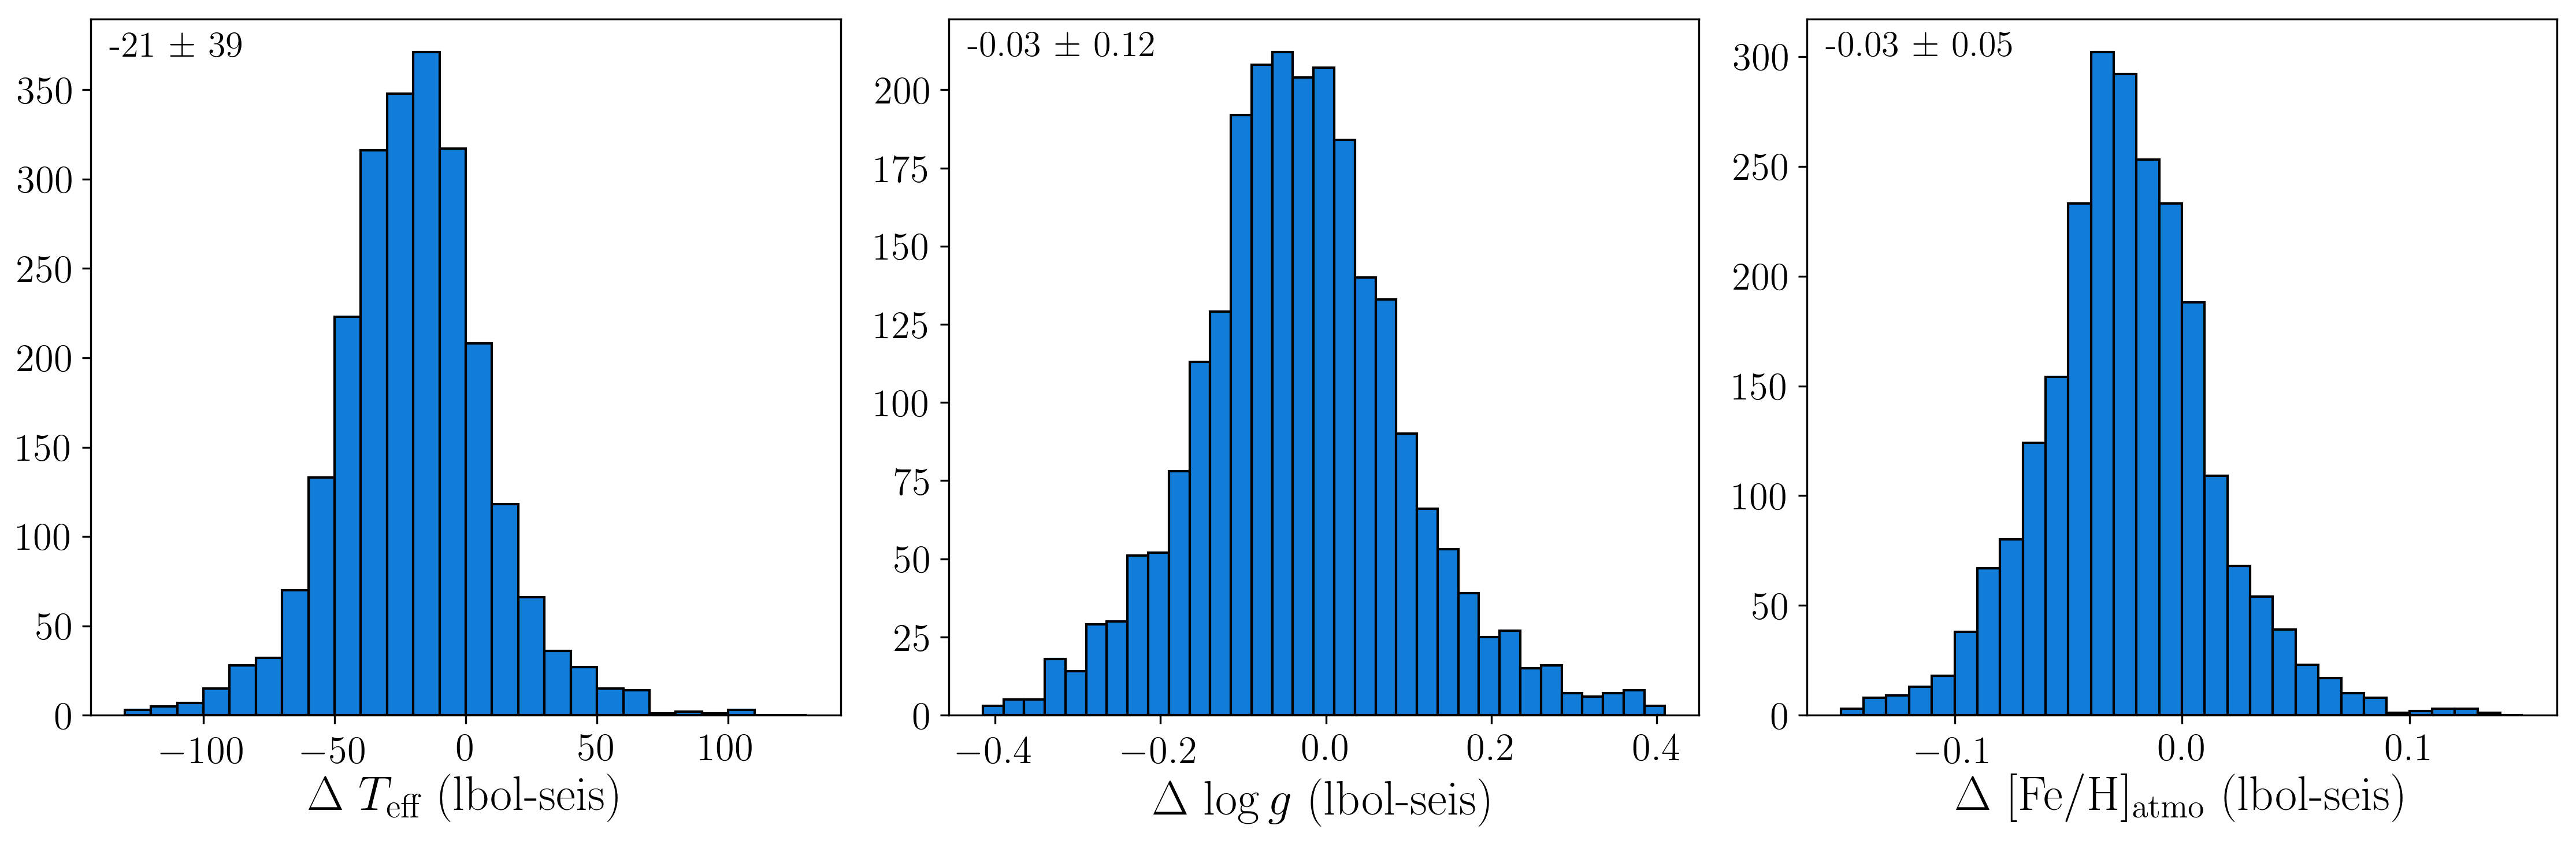
\includegraphics[width=\textwidth]{../../seis/figures/seis_setup_difference_lbol.png}
\caption{Differences (lbol - seis setups) of stellar parameters (left $T_\text{eff}$, middle $\log g$, right [Fe/H] for the stars with asteroseismic information.}
\label{fig:seis_comparison3}
\end{figure}

\subsection{Stars in clusters}

Based on the cluster membership analysis by Janez Kos, we have calculated the stellar parameters for all open and globular cluster members, for which an overview in forms of CMD, Kiel diagram, and distribution of [Fe/H] and interim ages (only maximum likelihood isochrone interpolation) can be found in \autoref{fig:cluster_overview}.

\begin{figure}[!ht]
\centering
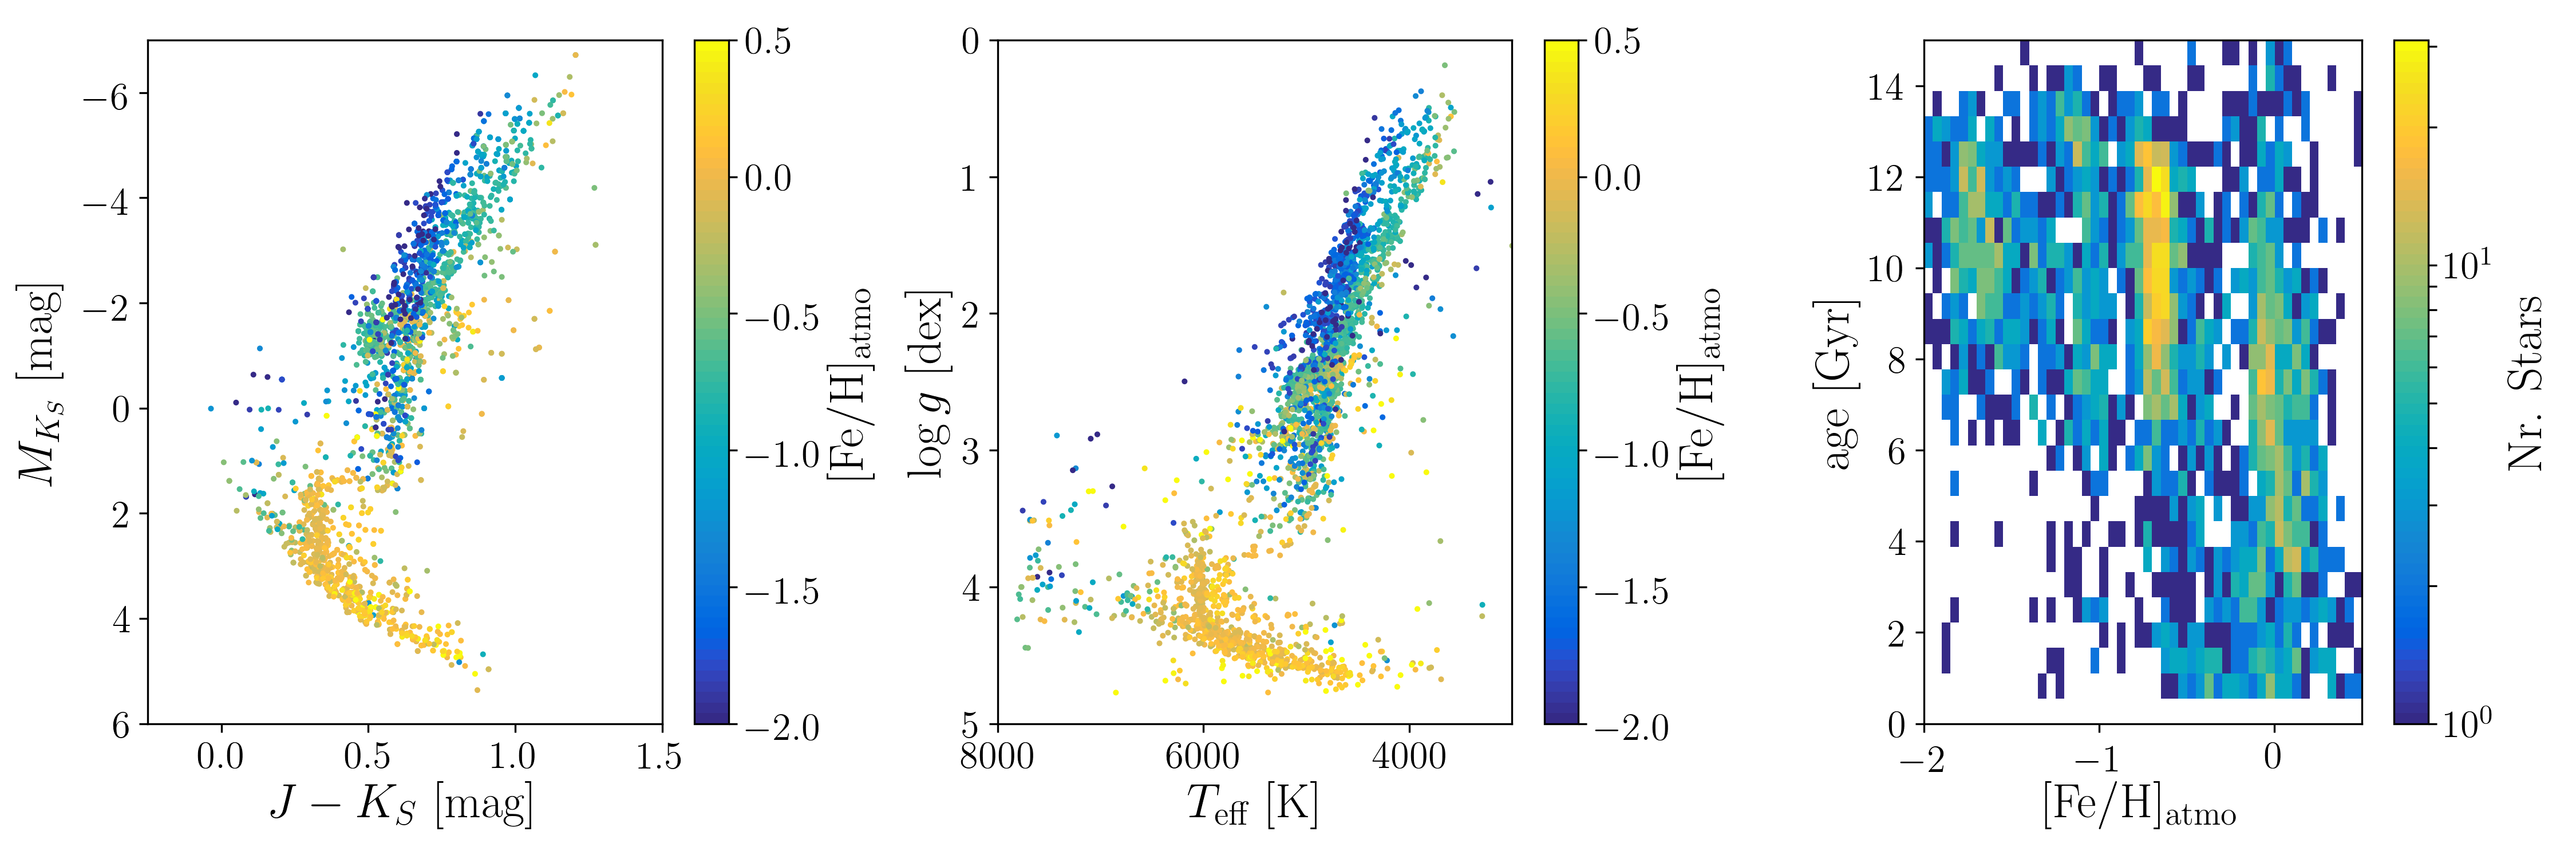
\includegraphics[width=\textwidth]{../../clusters/figures/CMD_Kiel_FehAge.png}
\caption{Overview of cluster stars observed by GALAH.}
\label{fig:cluster_overview}
\end{figure}

\section{Additional information: Dynamics}

Sven Buder has calculated velocities and actions for all observed GALAH stars based on the \textit{Gaia} DR2 5D information and the radial velocities from WG3 (GUESS).

The \href{https://github.com/svenbuder/GALAH_DR3/blob/master/dynamics/calculate_orbits.ipynb}{python script} is added added to the github repository and based on the following definitions:
\begin{itemize}
\item Uses Galpy 1.4  and its MWPotential2014
\item Position of the sun: $R_{GC,\odot} = 8.2\,\mathrm{kpc}$, $z_{GC,\odot} = 25\,\mathrm{pc}$ (Bland-Hawthorn \& Gerhard 2016)
\item $V_{LSR} = (-11, 10, 7.25)\,\mathrm{km/s}$ (Schoenrich+2012)
\item Errors are MC sampled with 10000 draws, distance is sampled with 2-sided Gaussian sampling the distance estimates from Bailer-Jones+2018
\item Calculated parameters: $X / Y / Z$, $U / V / W$, $R / \phi / z$, $J_R / L_Z / J_Z$, $e / z_\text{max} / R_\text{peri} / R_\text{ap}$ with means and standard deviations from MC sampling
\item Use the estimated values $e / z_\text{max} / R_\text{peri} / R_\text{ap}$ with caution! More testing and confirmation is needed!
\end{itemize}

\begin{figure}[!ht]
\centering
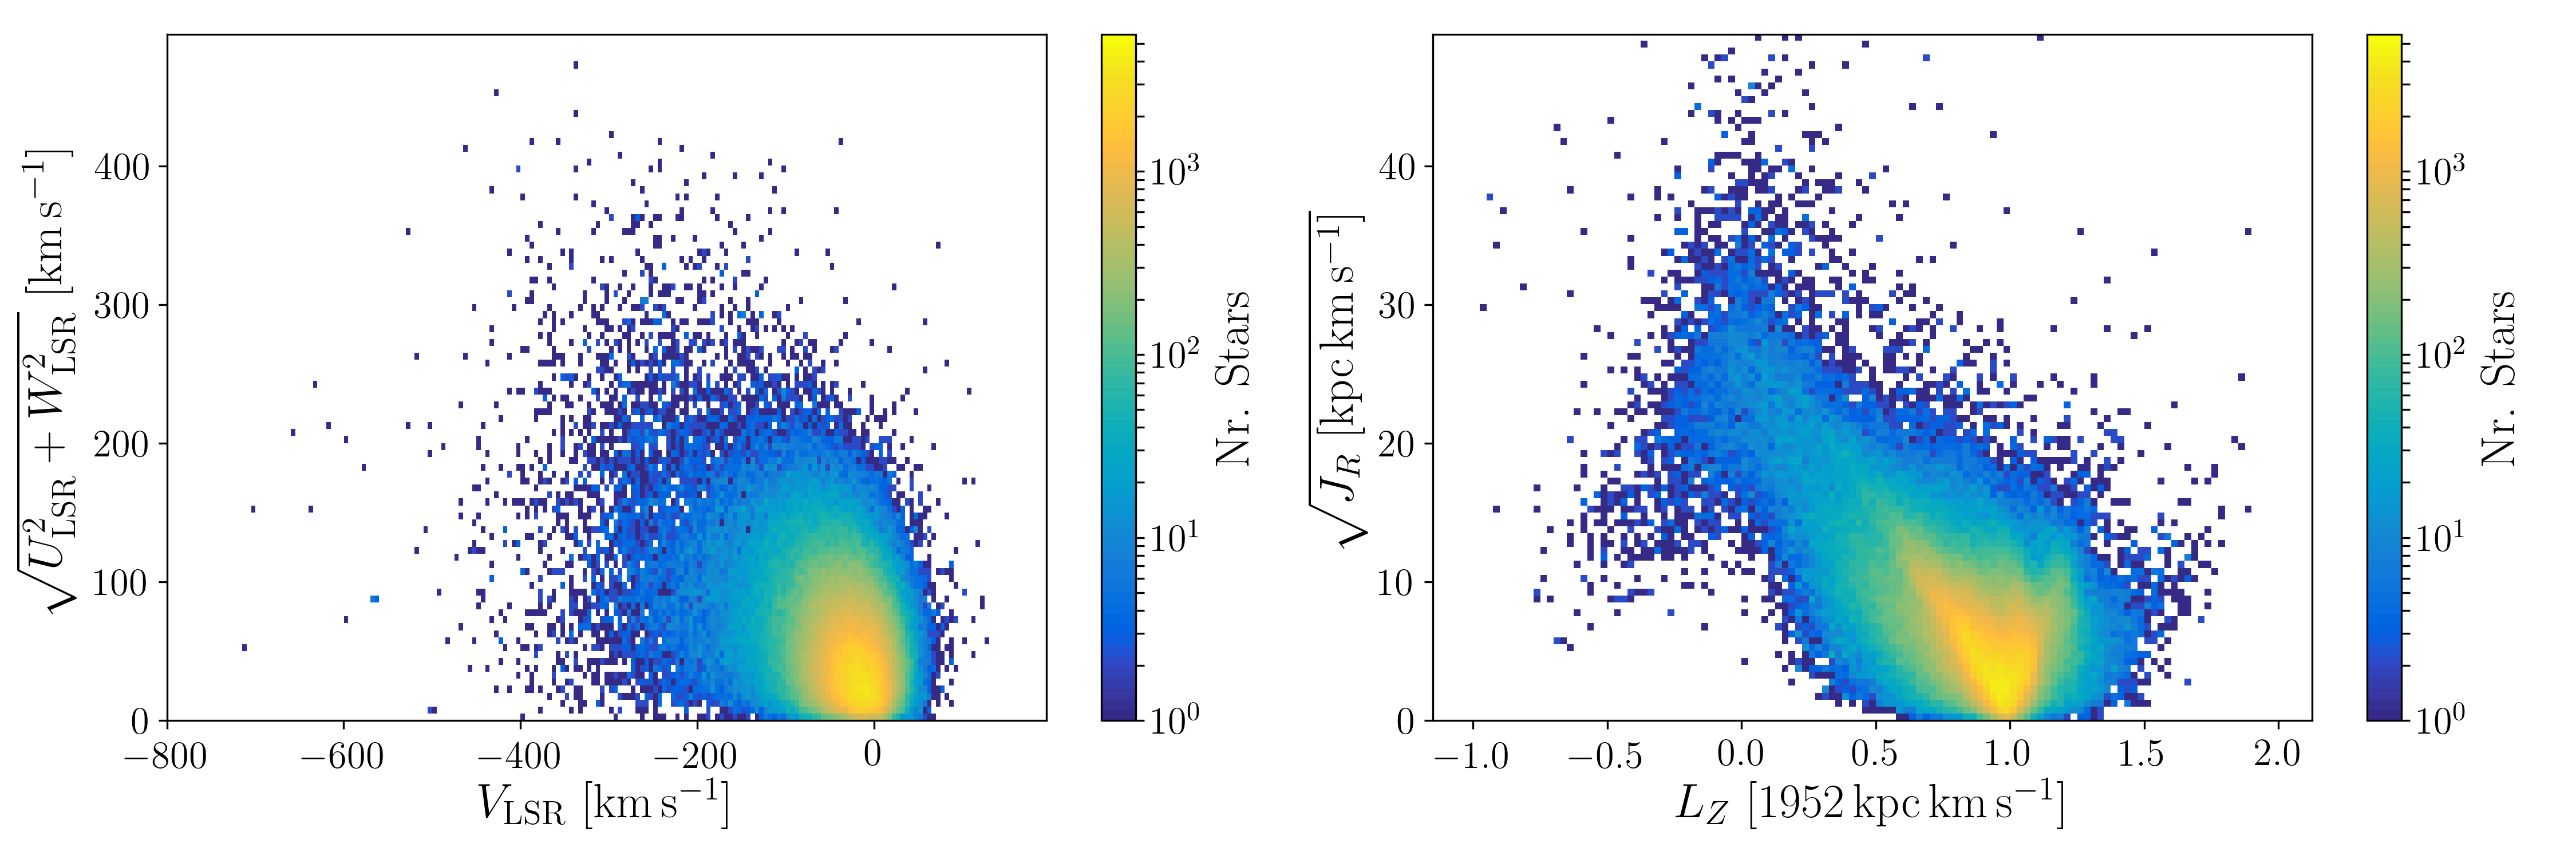
\includegraphics[width=\textwidth]{../../dynamics/figures/action_overview_clean_all.png}
\caption{Overview of dynamics of stars observed by GALAH.}
\label{fig:dynamics_overview}
\end{figure}

\begin{figure}[!ht]
\centering
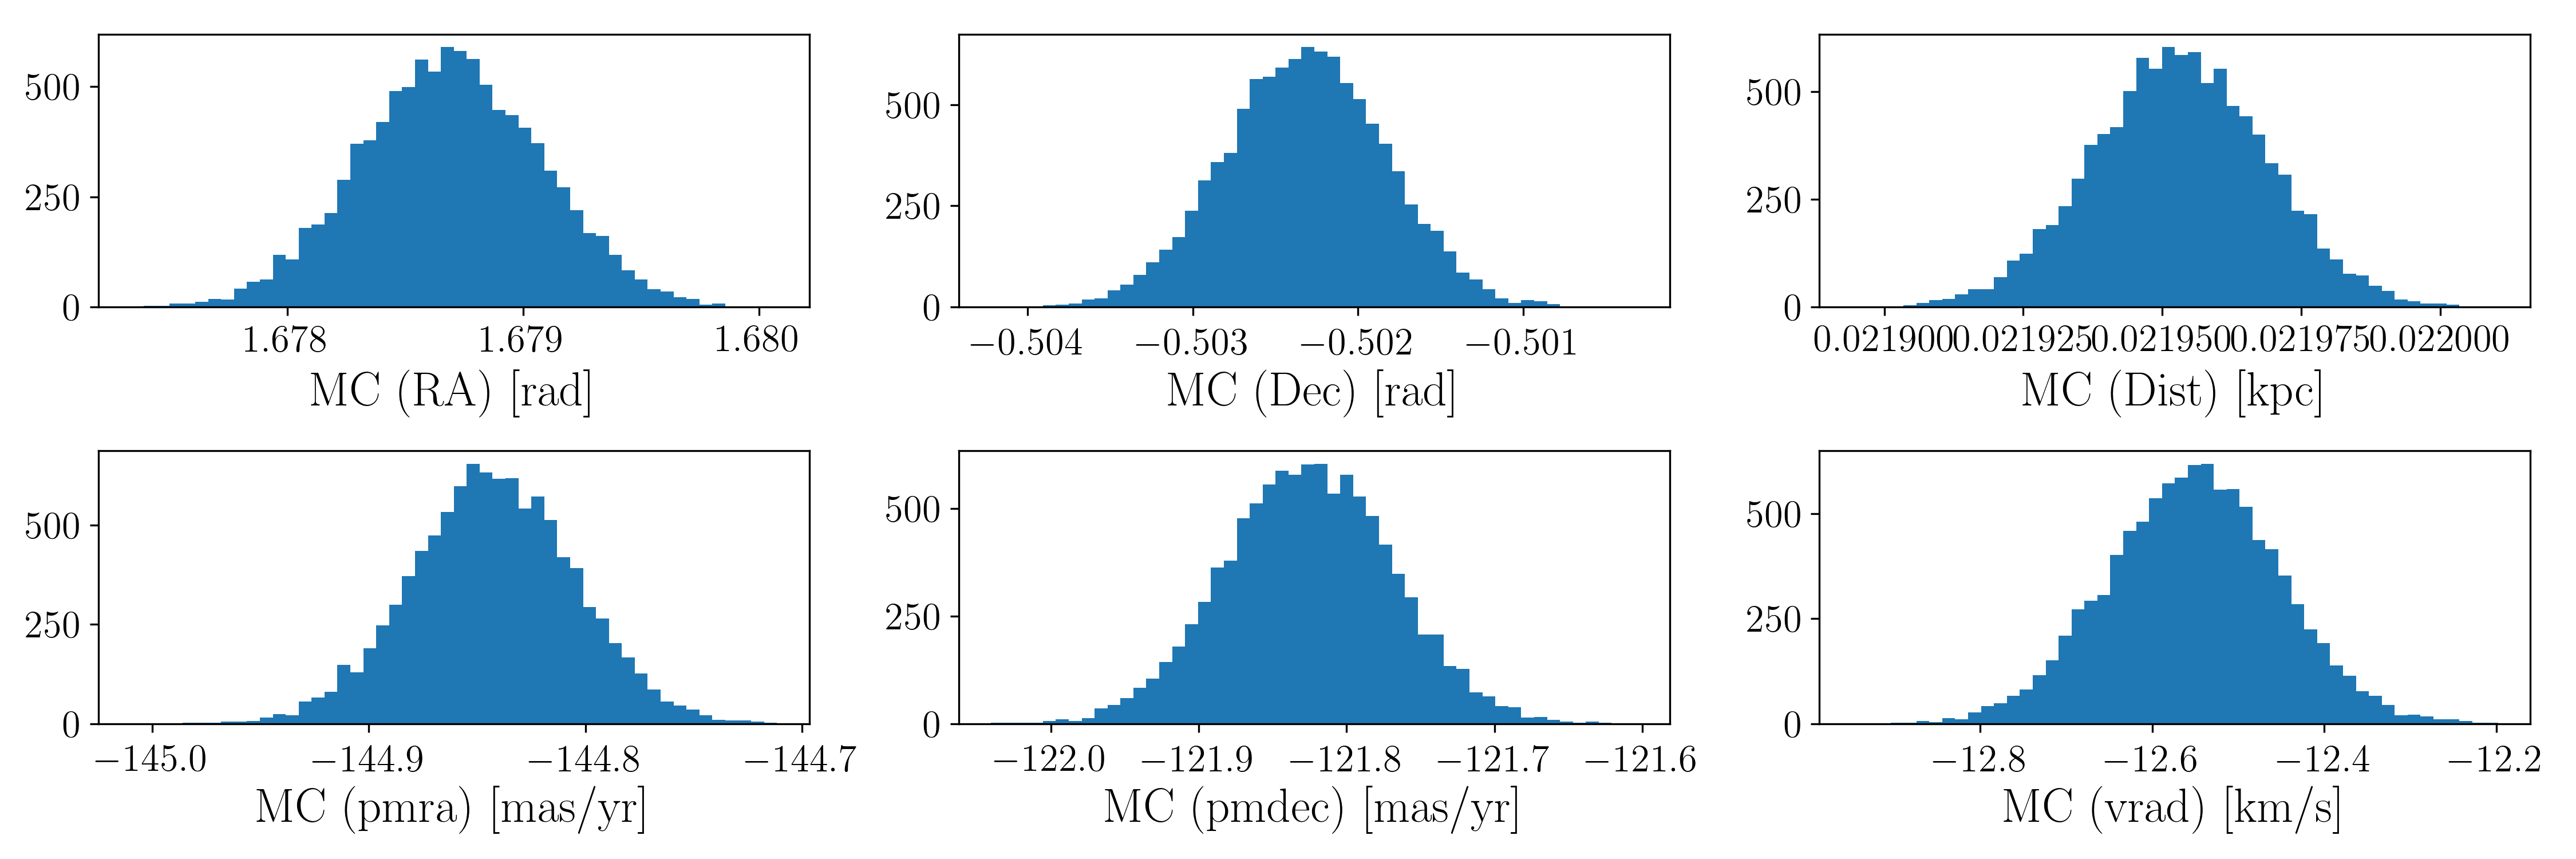
\includegraphics[width=\textwidth]{../../dynamics/figures/MC_input.png}
\caption{Diagnostic plots of dynamic output from a subset of the GALAH sample.}
\label{fig:dynamics_output}
\end{figure}

\begin{figure}[!ht]
\centering
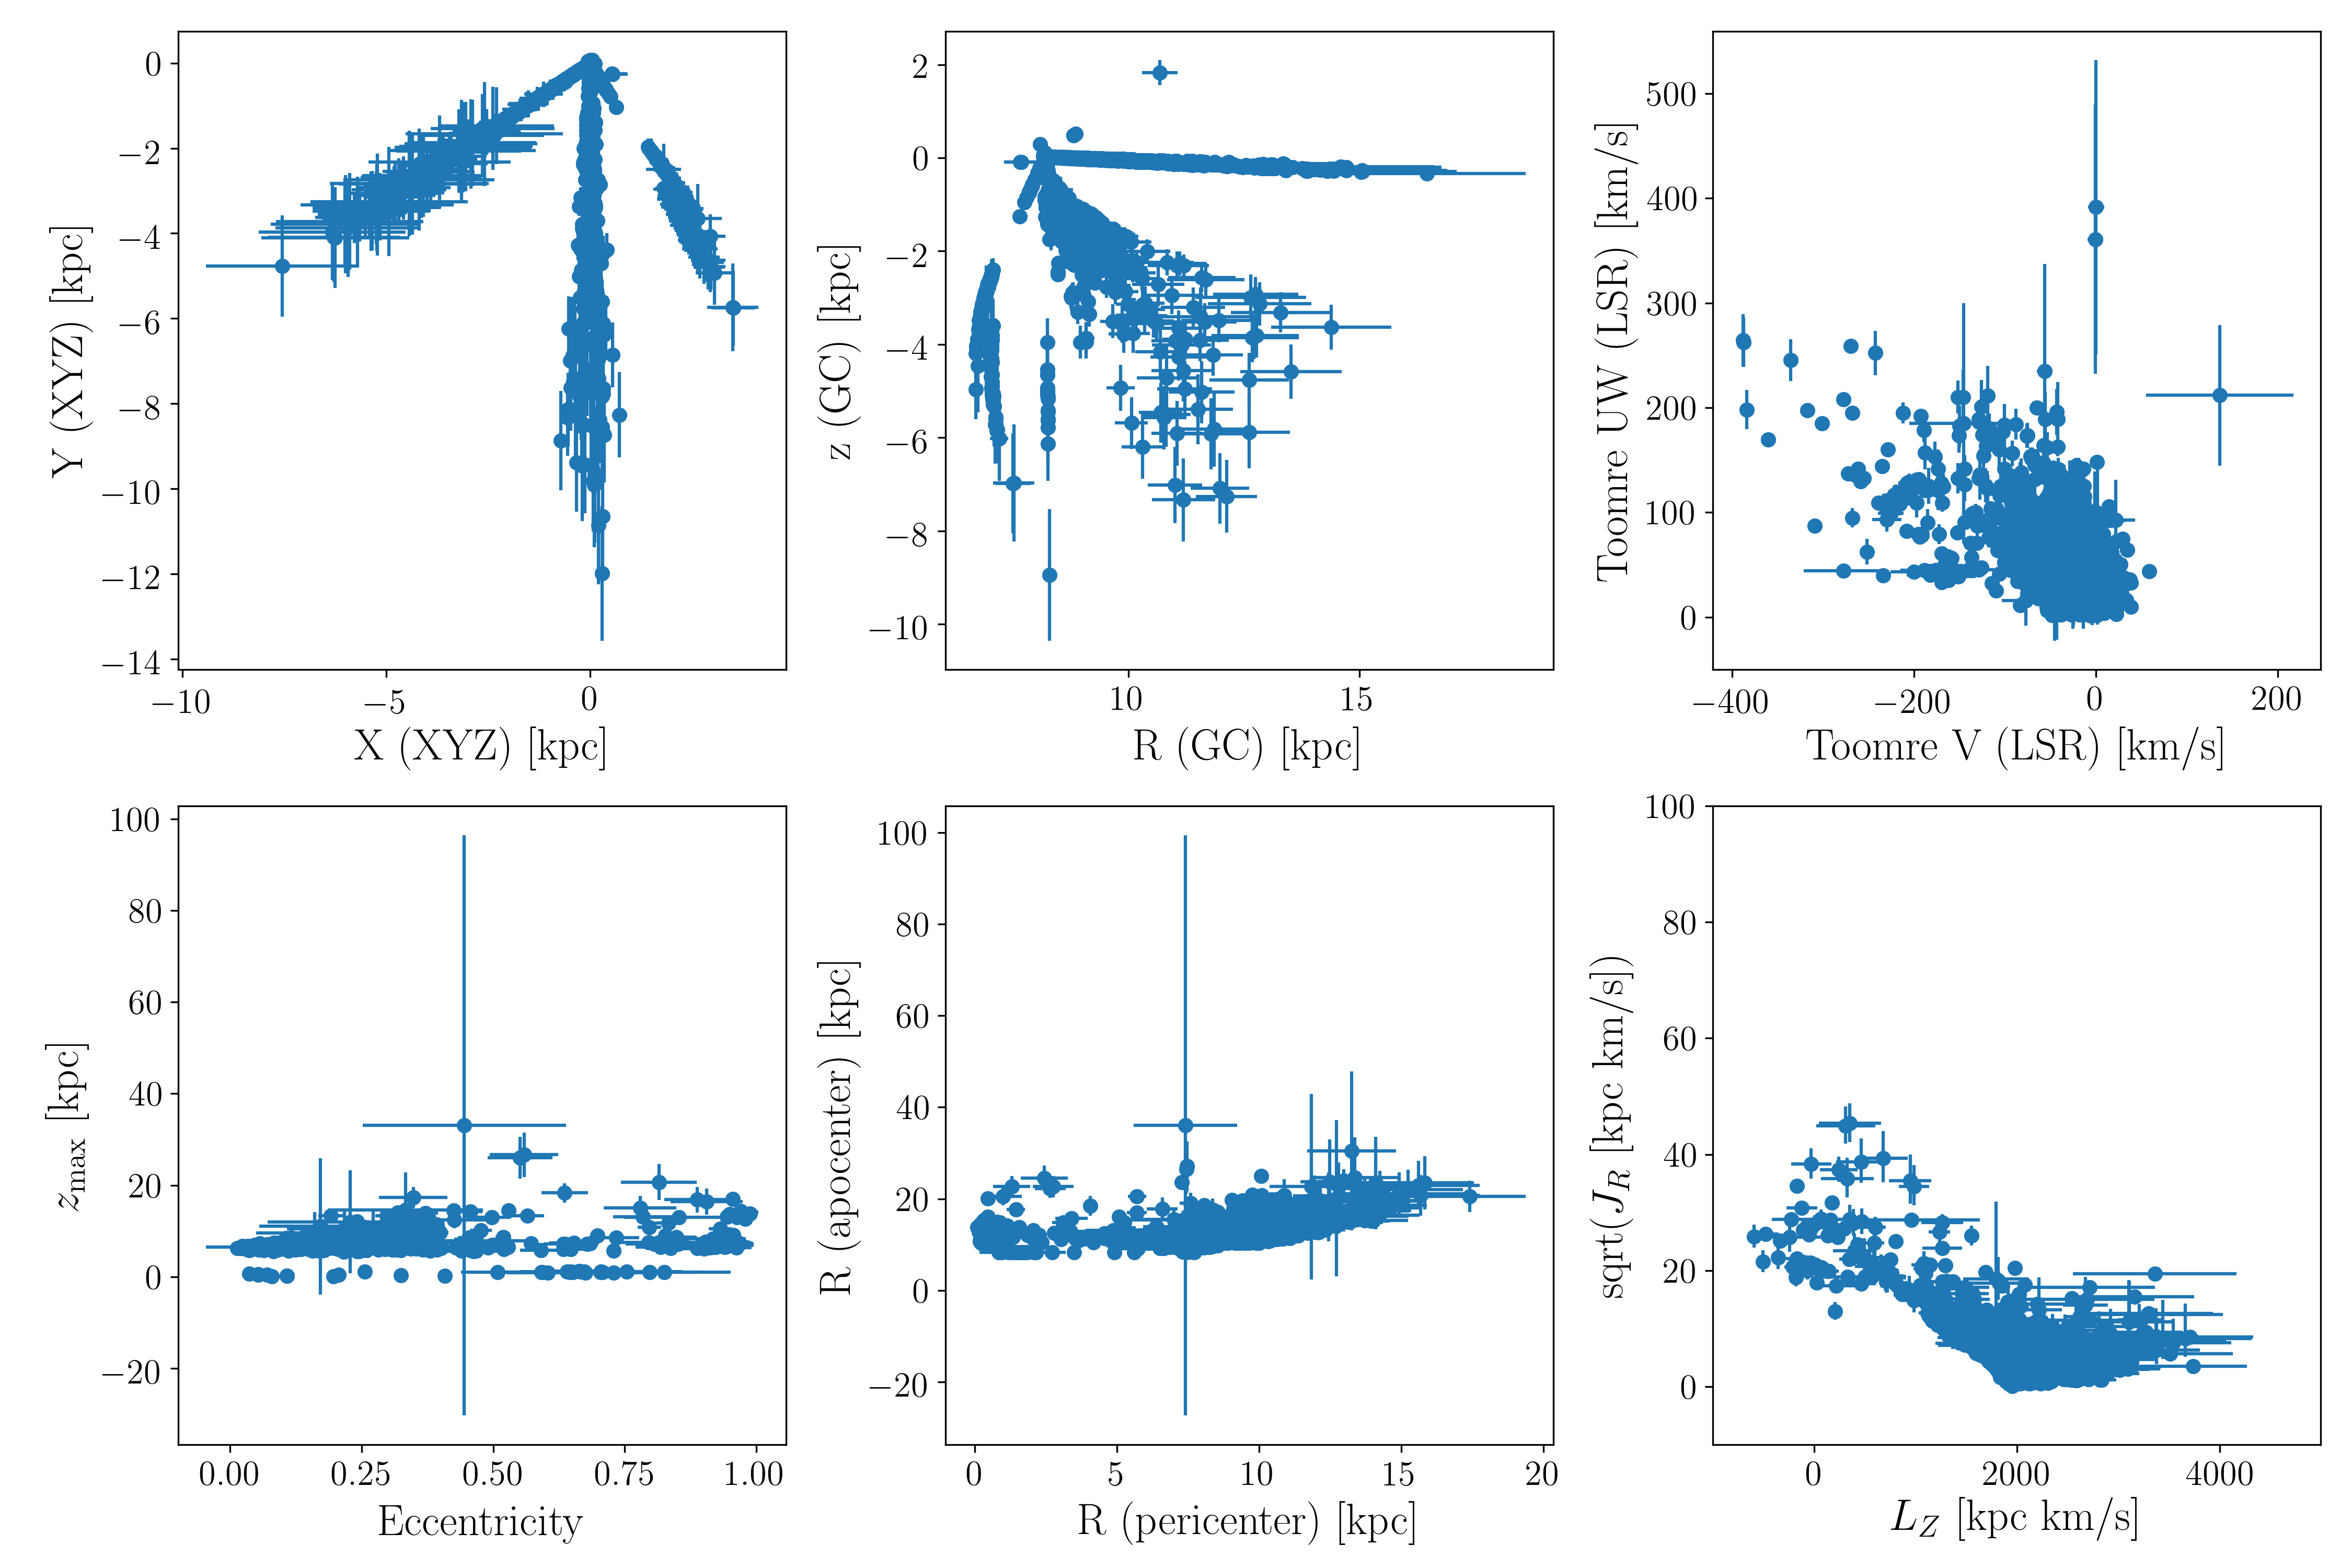
\includegraphics[width=\textwidth]{../../dynamics/figures/MC_output.png}
\caption{Diagnostic plots of dynamic output from a subset of the GALAH sample.}
\label{fig:dynamics_input}
\end{figure}

\end{document}